\documentclass[phd,oneside,11pt,norunningheaders]{ubcthesiscpbl}%[phd,10pt,noupper,runningheaders]{ubcthesis} 
\usepackage[utf8]{inputenc}  
\usepackage{setspace}
\newcommand{\ifdoDoubleSpace}[1]{}
% committee option is for draft: 1.5 spacing
\setcounter{secnumdepth}{4}
\setcounter{tocdepth}{4}
%\makeatletter

\if@twoside
\def\setpageforTOC{\setcounter{page}{2}}
\else
\def\setpageforTOC{}
\fi

\if@twoside
  \def\ps@plain{%
    %\let\@oddfoot\@empty\let\@evenfoot\@empty
    \let\@oddhead\@empty\let\@evenhead\@empty
    %\def\@evenhead{%
    \def\@evenfoot{%
      \parbox{\textwidth}{%
        \makebox[\textwidth]{{\pagenumberfont\thepage}\hfill}
        %\if@headline\vspace{\headlinespace}\fi
        }%
    }%
    %\def\@oddhead{%
    \def\@oddfoot{%
      \parbox{\textwidth}{%
        \makebox[\textwidth]{\hfill{\pagenumberfont\thepage}}
        %\if@headline\vspace{\headlinespace}\fi
      }%
    }%
    }%
\fi


  \def\ps@plain{%
    %\let\@oddfoot\@empty\let\@evenfoot\@empty
    \let\@oddhead\@empty\let\@evenhead\@empty
    %\def\@evenhead{%
    \def\@evenfoot{%
      \parbox{\textwidth}{%
        \makebox[\textwidth]{{\pagenumberfont\thepage}\hfill}
        %\if@headline\vspace{\headlinespace}\fi
        }%
    }%
    %\def\@oddhead{%
    \def\@oddfoot{%
      \parbox{\textwidth}{%
        \makebox[\textwidth]{\hfill{\pagenumberfont\thepage}}
        %\if@headline\vspace{\headlinespace}\fi
      }%
    }%
    }%


\makeatother
\usepackage{phdthesis}
\usepackage{mathptmx} 
\setcounter{secnumdepth}{4}
\setcounter{tocdepth}{4}
\usepackage{varioref} % eqref is in here?????

\usepackage{url} % For a url..
\usepackage{amssymb} % amssymb/amsmath have?? checkmark? eqref?
\usepackage{amsmath} % align environment (everyone says stop using eqnarray!)


\usepackage{index}
% Following two are just black holes to accomodate index calls in the
% variable list table
\newindex{vars}{vidx}{and}{Coded variables}
\newindex{surveyvars}{sidx}{sand}{Survey variables}

\providecommand{\tabularnewline}{\\} % LyX relic

%******** natbib ********************************
% This is a very nice package for bibliographies.  It includes options
% for sorting and compressing bibliographic entries.
\usepackage[square,authoryear]{natbib} % REMOVED OPTIONS: numbers,sort&compress,

% cPbL: For chapter-level bibliographies:
\usepackage{bibtopic}
\bibliographystyle{aguCpbl}%cje}

%******** graphics and graphicx ******************************
% This allows you to include encapsulated postscript files.  If you
% don't have this, comment the \includegraphics{} line following the
% comment "%includegraphics" later in this file.
\usepackage{graphicx}

%******** lscape ******************************
% This allows you to include landscape layout pages by using the
% |landscape| environment. Note that this output might only be valid
% after converting to a postscript or pdf file.
\usepackage{lscape}

%******** psfrag ******************************
% This allows you to replace text in postscript pictures with formated
% latex text.  This allows you to use math in graph labels
% etc. Uncomment the psfrag lines following the "%psfrag" comment
% later in this file if you don't have this package.  The replacements
% will only be visible in the final postscript file: they will be
% listed in the .dvi file but not performed.
\usepackage{psfrag}

%******** afterpage ***************************
% This package allows you to issue commands at the end of the current
% page.  A good use for this is to use the command
% \afterpage{\clearpage} right after a figure.  This will cause the
% figure to be inserted on the page following the current one (or on
% the current page if it will fit) but will not break the page in the
% middle.
\usepackage{afterpage}

%%%%%%%%%%%%%%%%%%%%%%%%%%%%%%%%%%%%%%%%%%%%%%%%%%%%%%%%%%%%%%%%%%%%%%
% Allow a new preface entity which is useful for a DEDICATION
%%%%%%%%%%%%%%%%%%%%%%%%%%%%%%%%%%%%%%%%%%%%%%%%%%%%%%%%%%%%%%%%%%%%%%
% Use as follows:
%     \beforepreface
%     \dedication{To my grandparents ...}
%     \prefacesection{Abstract}   ...
%
% 2000 February 14: cPbL
\def\dedication#1{
  \chapter[Dedication]{} % Put in TOC but don't display "Dedication"
                         % on page
%  \thispagestyle{empty}  % No page number
  \thispagestyle{plain}   % Yes page number
  \vspace{6cm}
  \begin{center}
    #1
  \end{center}
  }
     
% Define a command to start a bib section for manuscript-based thesis
\newcommand{\placeSecBib}[1]{
\forThesis{
\newpage
\begin{btSect}{veblen,evolution,institutions,swb,general,urban,weather,sk} 
\chapter*{Bibliography for #1} 
\addcontentsline{toc}{section}{Bibliography for #1}
\btPrintCited 
\end{btSect} 
\end{btUnit}
}
}

%\renewcommand{\listfigurename}{List of figures}
%\renewcommand{\listtablename}{List of tables}

 
% These commands are optional.  The defaults are shown.
%\institution{The University Of British ColumbiaV}
%\institutionaddress{Vancouver, Canada}
\program{Economics}

% You can issue as many of these as you have...
\previousdegree{S.B. Physics, Massachusetts Institute of Technology, 1995}
\previousdegree{M.Sc. Applied Physics, Stanford University, 1998}
\previousdegree{Ph.D. Applied Physics, Stanford University, 2001}


% These commands are required.
\title{Geography, reference groups, and the determinants of life satisfaction}
\subtitle{}
\author{Christopher Paul Barrington-Leigh}
\copyrightyear{2009} 
\submitdate{January 2009}%\today}

\advisor{Thomas Lemieux}
\advisortitle{Professor of Economics}
% One might want to override the format of the section and chapter
% numbers.  This shows you how to do it.  Note that
\renewcommand\thepart         {\Roman{part}}
\renewcommand\thechapter      {\arabic{chapter}}
\renewcommand\thesection      {\thechapter.\arabic{section}}
\renewcommand\thesubsection   {\thesection.\arabic{subsection}}
\renewcommand\thesubsubsection{\thesubsection.\arabic{subsubsection}}
\renewcommand\theparagraph    {\thesubsubsection.\arabic{paragraph}}
\renewcommand\thesubparagraph {\theparagraph.\arabic{subparagraph}}

\usepackage{relsize}
\newcommand\muchsmaller{\smaller\smaller}

\usepackage{cpblRef}
\usepackage{cpblTables}


% Below is for the data (survey appendix). Gods help me!
\usepackage{psfrag,color,graphicx}
\graphicspath{{/home/cpbl/papers/incomeCMA/plots/}{./}}

\graphicspath{{/home/cpbl/models/veblenNeighbourhoods/figuresLEL/}{/home/cpbl/models/veblenNeighbourhoods/figuresvs/}{./}{./figuresvs}{./tmpg}{/home/cpbl/papers/incomeCMA/plots/}{./}}
\usepackage{amsthm}
\usepackage{ushort} % For an underbar that looks like \bar.
\usepackage{wrapfig} % For acknowledgements only

% BELOW DEFINES THE THEOREM ENVIROS I NEED: PROPOSITION, LEMMA, PROOF

\newtheorem{theorem}{Theorem}[section]
\newtheorem{lemma}[theorem]{Lemma}
\newtheorem{proposition}[theorem]{Proposition}
\newtheorem{corollary}[theorem]{Corollary}

\newenvironment{definition}[1][Definition]{\begin{trivlist}
\item[\hskip \labelsep {\bfseries #1}]}{\end{trivlist}}
\newenvironment{example}[1][Example]{\begin{trivlist}
\item[\hskip \labelsep {\bfseries #1}]}{\end{trivlist}}
\newenvironment{remark}[1][Remark]{\begin{trivlist}
\item[\hskip \labelsep {\bfseries #1}]}{\end{trivlist}}

% Some tools to differentiate between thesis version and journal
% manuscript version.
\newcommand{\forThesis}[1]{#1}
\newcommand{\forPaper}[1]{}



\newcommand{\LELcfig}[1]{\includegraphics[width=0.75\textwidth,keepaspectratio]{#1.\epspdf}}%{\input{#1}.tex}
% Above redundant: see cpblRef.sty LELwfig


\newcommand{\epspdf}{pdf}%{eps}%
\newcommand{\cmykrgb}{cmyk}%{rgb}
\newcommand{\rawplotspath}{/home/cpbl/models/veblenNeighbourhoods/plots/raw/}
\newcommand{\iCMArawplotspath}{/home/cpbl/econ/favouritePlots/cityScatterPlots/}%{papers/incomeCMA/plots/raw/}
\usepackage[footnotesize,bf]{caption} % Does this actually call caption2 or caption3?
\setlength{\captionmargin}{20pt}


% Inconspicuous hyperref -- very nice.
  \usepackage[   
       colorlinks,
      citecolor=black,
       filecolor=black,
       linkcolor=black,
       urlcolor=black  
   ]{hyperref}



\newif\ifNBER

%%% TURN OFF COMMENTS:
\renewcommand{\draftComment}[1]{}
\renewcommand{\safeDraftComment}[1]{}
\renewcommand{\cpblOldComment}[1]{}

% Turn on comments:

%\renewcommand{\draftComment}{\draftCommentColouredBox}
%\renewcommand{\cpblOldComment}{\draftCommentColouredBox}
 
% UBC has strange format requirements, but some things not strict. So
% don't worry about things looking nice. Widen so I can fit my big tables:
% To ensure that the margin fiddling for the huge/wide/long tables
%\addtolength\oddsidemargin{-1cm}
%\addtolength\evensidemargin{-1cm}
%\addtolength\textwidth{2cm}
\addtolength\oddsidemargin{-1cm}
\addtolength\evensidemargin{-1cm}
\addtolength\textwidth{2cm}

\newcommand{\starsOrColours}[2]{#1}

\ifdoDoubleSpace{\doublespacing}
\begin{document}
%\renewcommand\baselinestretch{1.0}

\ifdoDoubleSpace{ \begin{singlespace} }

% This starts numbering in Roman numerals as required for the thesis
% style.
\frontmatter

% The order of the following components is preserved.  The order
% listed here is the order currently required by the library.
\maketitle
\newpage\thispagestyle{empty}\newpage  %\pagestyle{empty}
\begin{abstract} %\pagestyle{plain}
\setcounter{page}{2}

This dissertation combines three contributions to the literature on
the determinants of well-being and the social nature of preferences....


\end{abstract}
\newpage\thispagestyle{empty}\newpage  %\pagestyle{empty}
\setpageforTOC


\tableofcontents
%\listoftables
%\listoffigures

\chapter{Acknowledgements}
This is to thank those for whose support and criticism I could constantly count on
while working on my thesis. I will list them in alphabetical order:

\begin{itemize}
\item My parents thanks who I had the chance to study and who always believed in me.  
\item Dh.D. Andrzej Głowacz for his advices. 
\item Anna Pawłowicz thanks who I had the best motivation ever and I could always count on.
\end{itemize}

Thank You all very much!

\emph{Special mention:} Thanks to the people whose work I used while working on my project.
Thanks to all for who Open Source became a pattern for developing software.



\dedication{\Large \em
For Iris: this one --- and I promise it's the last --- is for you,\\
who set me on this hidden path in 2000,\\ \vspace{5mm}
And in memory of Robert, who had so much left to say.
}

% Force a new page.
\newpage


% Suppress the running headers for this page only.
\thispagestyle{plain}

% Now regular page numbering begins.
\mainmatter%



\ifdoDoubleSpace{ \end{singlespace} }
\setcounter{secnumdepth}{4}
\setcounter{tocdepth}{4}
%\chapter{Introduction}
\label{sec:Introduction}
Creating a network applications in nowadays might be a complicated process of design which involves long series of research and experiments or be a fairly simple procedure that does take only tenth of it time and effort. In both cases the frequent evaluation metric is the application scalability more than thousands line of code or model complexity. With time gained popularity network  applications usage arises what in consequence implies increase in frequency that application is requested to serve its functionality. This growth can be calculated and included at the is planing level becoming a good programming practice that places itself close to other already widely approved design patterns. With no doubt scalability is staring to play a more and more important role being often set at the same level with such issues like portability or security[quote]. I was looking for idea for an application that by its original functionality would heave the potential to become with time a really heavy traffic network application with lots of active users.

\section{Popular notes taking applications}\label{sec:popular_apps} 
blablabla
\subsection{Appx}\label{subsec:x} 
\subsection{Appy}
\section{Popular Version Control Systems}\label{sec:popular_vcs}
\subsection{Mercurial}
\subsection{Comparison}
\section{Scalability}\label{sec:scalability}
\section{Role of programming languge}\label{sec:language}
\subsection{Python}
\subsection{Comparison}

%%%%%%%%%%%%%%%%%%%%%%%%%%%%%%%%%%%%%
\chapter{Introduction}
\label{sec:Introduction}
Creating a network applications in nowadays might be a complicated process of design which involves long series of research and experiments or be a fairly simple procedure that does take only tenth of it time and effort. In both cases the frequent evaluation metric is the application scalability more than thousands line of code or model complexity. With time gained popularity network  applications usage arises what in consequence implies increase in frequency that application is requested to serve its functionality. This growth can be calculated and included at the is planing level becoming a good programming practice that places itself close to other already widely approved design patterns. With no doubt scalability is staring to play a more and more important role being often set at the same level with such issues like portability or security[quote]. I was looking for idea for an application that by its original functionality would heave the potential to become with time a really heavy traffic network application with lots of active users.

\section{Popular notes taking applications}\label{sec:popular_apps} 
blablabla
\subsection{Appx}
\subsection{Appy}
\section{Popular Version Control Systems}\label{sec:popular_vcs}
\subsection{Mercurial}
\subsection{Comparison}
\section{Scalability}\label{sec:scalability}
\section{Role of programming languge}\label{sec:language}
\subsection{Python}
\subsection{Comparison}

\chapter{Introduction}
\label{sec:Introduction}
Creating network applications nowadays might be a complicated process of design which involves long series of research and experiments or, on the other hand, it might be a fairly simple procedure that takes only a tenth of its time and effort. In both cases, the most frequent evaluation metric is the scalability of the application, more than a thousand of lines of code or the complexity of the model. With the rise in popularity, the usage of network applications increases, which in consequence results in an increase in the frequency that the application is requested to serve its functionality. This growth can be calculated and included at the planning level, thus becoming a good programming practice that places itself close to other widely approved design patterns. With no doubt is scalability starting to play a more important role, being often set at the same level with such issues like portability or security[quote]. The present thesis aims to introduce an application that by its original functionality would heave the potential to become a heavy traffic network application with numerous active users. In this chapter the reader can find an overview of popular notes taking applications, understand the basis of Version Control Systems, and learn about more technical sections regarding the Python programming language as well as terms of scalability in a Google App Engine product. 
\chapter{System Concept}\label{chap:concept}
The following chapter will cover the system concept, the functionality it offers and the general functional system description. Also, the following sections should clarify how the SmartNotes application can be used, illustrate its design using the UML diagrams and prepare the reader for more detailed system description included in the chapter~\ref{chap:sys_description}.

The idea of SmartNotes has been inspired by the Google Notebook application which was being actively developed until January 2009, when Google announced that further development work on this project is stopped. Google Notebook has an interesting interface and features, some of them already motioned in section~\ref{subsec:google_notebook}. what was still missing from the functionality until January 2009 was comfortable notes usage without network connectivity. The aim of the subject of the thesis was to use the idea of making a truly scalable notes taking application that would be even more flexible.

\section{Functionality description}\label{sec:functionality_descr} 
Detailed description of how a system may be used should by of utmost importance both to the developer and to the end user, as it helps gain a general perspective, called 10,000-foot view\cite[page 49]{uml_use_case}, of the system and make useful observations. The implementation as well as the conceptual and system design decisions become a side issue, as the foreground is always occupied by the functionality  the application is to offer. For that reason, the use of case scenarios and flow charts will be very helpful in describing the efficient way of using the SmartNotes application.

Users willing to work on their notes disregarding network connectivity will need to install iSmartNotes, which is a graphical interface of SmartNotes. Specifically, the SmartNotes application is divided into the web-based system and the graphical desktop interface, a separation with which UI experiments can be done without the need of having the web browser open in order to work on the notes. The web based part of SmartNotes makes the synchronization feature possible and allows to monitor the entire system of SmartNotes. However, in order to use the synchronization feature, the iSmartNotes needs to be activated by the user. Additionally, since users of SmartNotes are expected to have a Google account\footnote{Creating a Google account by visiting \url{https://www.google.com/accounts/} gives a access to various services offered by the Google company where Gmail, Google News or Google Finance are one of the most popular tools. These are regarded secure and solid services users can relay on.} the activation code will be available after logging in to the SmartNotes system with that account. This process is illustrated on figure~\ref{fig:ismartnotes_activation}. The idea behind it is to make the use of the popular Google Account and not multiply the accounts to services that the user has to know the login and password. Basing on the activation key, the user is granted access to his personalized SmartNotes account and to the synchronization feature. Without the activation, iSmartNotes can be used as a regular notes editor.  
\begin{figure}[ht]
\begin{center}
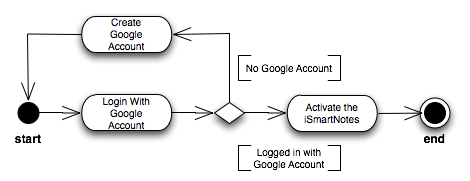
\includegraphics[scale=0.65]{charts/activate_iSmartNotes.png}
\caption{The iSmartNotes application activation with the Google Account.}
\label{fig:ismartnotes_activation}
\end{center}
\end{figure}
The skim of functionality offered by iSmartNotes is demonstrated on figure~\ref{fig:workon_ismartnotes}.
\begin{figure}[ht]
\begin{center}
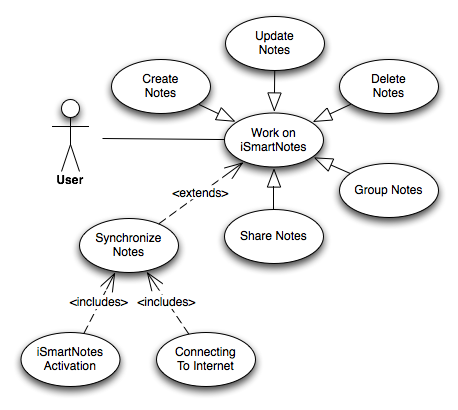
\includegraphics[scale=0.55]{charts/work_on_iSmartNotes.png}
\caption{The iSmartNotes application use cases.}
\label{fig:workon_ismartnotes}
\end{center}
\end{figure}
This includes the CRUD operations and three extra features. Firstly, the notes can be easily grouped together in named tabs, which should make organizing and finding notes much easier. Secondly, it is possible to publish the notes marked as shared. The final feature is the synchronization process that requires iSmartNotes activation and network connection to contact with the web-based part of SmartNotes. What remains to be discussed is the cooperation between iSmartNotes and the web-based part of SmartNotes, therefore, the relation between them and the functionality offered to the user and administrator are shown on figure~\ref{fig:ismartnotes_smartnotes}. 
\begin{figure}[ht]
\begin{center}
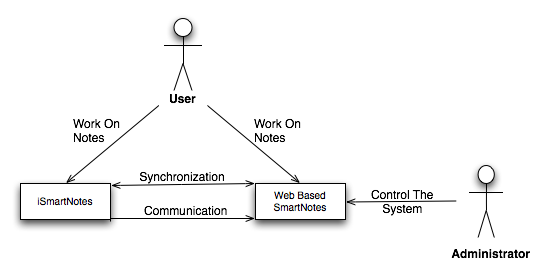
\includegraphics[scale=0.55]{charts/iSmartNotes_SmartNotes.png}
\caption{The cooperation of iSmartNotes and web based SmartNotes.}
\label{fig:ismartnotes_smartnotes}
\end{center}
\end{figure}

This interesting concept allows the user to work on iSmartNotes as well as the Web-based part of SmartNotes exchangeably, at the same time letting the SmartNotes application care for work synchronization, which has been also highlighted in the above discussed picture. Yet, however functional and elastic the application may seem, the same functionality is not feasible in the web interface of the present project, even if the administrator is granted access to tools like datastore data browser, system status or application dashboard described in section~\ref{sec:gae_general}. This can help to quickly diagnose faults within the application and rollback it to the latest stable version. Moreover,  it can indicate that the rescuers are not sufficient to serve the traffic and eventually extend them. The tools work effectively in cooperation with Google Webmaster Tools and the Google Analytics as they can provide more information concerning the web page and its visitors.

It appears to be worth describing the synchronization feature in more detail. The feature is realized by the VCS which was introduced in section~\ref{sec:popular_vcs}. No matter if the user works online or not, they have full access to notes and synchronize them online. As it has been marked on the graph from figure~\ref{fig:ismartnotes_smartnotes}, the synchronization process is bidirectional: it is triggered from the web-based part of SmartNotes, which plays a role of the main server, and the iSmartNotes, playnig the role of clients and reverse. This type of set-up should allow to update the notes whenever necessary. Another point presented in figure~\ref{fig:ismartnotes_smartnotes} is the directional communication between iSmartNotes and SmartNotes, which should be understand as an additional logic allowing to perform operations on the user side by the help of iSmartNotes, including the display of user information on significant events like availability of new features or versions.  As a matter of fact, the process is directional in one way as it is the iSmartNotes application which receives the information from the SmartNotes server and displays it to the user. Whereas the presented functionality does not fully exploit the possible feature list, as mentioned in section~\ref{subsec:vcs_comparison}, it is a good practice to keep the application as simple as possible and focus on a set of clearly defined key features.

\section{Functional description}\label{sec:functional_descr}
The SmartNotes application should run on a infrastructure that can ensure complete availability and high load. Easy system maintenance and openness to future expansion in functionality are also strongly desirable features. It is not pointless to mention that the above requires resource usage, which makes the financial model of utmost importance and is the already introduced 10,000-foot view of system requirements. Adding a friendly deployment methodology and good documentation is what would satisfy the most demanding developer.

Admittedly, in order for the application to gain popularity, users should be well informed about the application and its functionality; also, it is vital to provide availability of instructions on how to get started. For these reasons, the landing page should be not only informal and practical, but also international to reach greater group of users.

From the architectural point of view, SmartNotes is a simple client-server application, the only difference being the usage of DVCS, which allows the machines to access thesame set of commands and make their hard disks hold the entire repository with its history. Yet, it may be confusing that it still remains a client-server architecture, but just as the centralized VCS do not recognize any other architecture than the client server, the distributed VCS uses it as one of possible use cases. In the following scenario one of the machines fulfills a role of the reverential server to which all remaining machines direct their requests, at the same time being a for of public repository with the most recent version that should be always available to users. In consequence, each client requires the installation of DVCS as one of the main components, while the size of the chosen VCS matters as much as its performance, which all in all has significant impact on the final performance of iSmartNotes. For optimum user experience, the iSmartNotes application provides an easy-to-install package that could be downloaded from the server serving static content, which is not only a faster solution from dynamically served content, but also allows to save system resources, costing a minimum of CPU time.

The next two sections state certain problems related to synchronization scenarios using VCS and the application activation. They will be analyzed focusing on the evaluating of a number of possible solutions and the argumentation will lead to the choice of the most optimal solution.  
 
\subsection{Synchronization scenarios using version control systems}\label{subsec:sync_scenarios}
It is one of the main responsibilities of version control systems to keep the repositories updated. Nevertheless they never perform update without a user request\footnote{This means that the user has to run an appropriate command or click on the right button when using a graphical interface. It could be naturally automated by writing a script that would perform that task for the user or by setting a cron job with a desired time interval, but the tool still requires the user to trigger the update process.}, the reasons for which are various, but dealing with conflict situations like the one shown on figure~\ref{fig:google_notebook} seams to be the most important. To put it in simple words conflict situation it is a situation when the VCS needs the user decision to resolve the conflict situation as it cant decide which from the concurring versions should be chosen. The way the merging is done differs with different version control systems but from the user perspective operations such like update and merge are quite easy to imagine. 

Due to lack of clarity in terminology including this basic operations of version control some additional explanations needs to be done. Mercurial implements \texttt{fetch} command  which includes three steps in the listed in  the order of execution:
\begin{enumerate}
\item{Lookup.}
\item{Getting changesets\footnote{Thist is a term used mainly in Mercurial related documentation to refer the data structures used for storing the differences between revisions. This seam to be more accurate then saying 'changes' or 'differences' and will be used in this document when concerning data structures.}.}
\item{Updating or merging.}
\end{enumerate}
The first two Mercurial implements as \texttt{pull} command and the last one has two commands called respectively \texttt{update} and \texttt{merge}. On the other side in the git system \texttt{fetch} does the same that Mercurial \texttt{pull} command and the git \texttt{pull} is a substitute for the \texttt{fetch} from Mercurial. To avoid confusion in the following document the terminology from the git system will be used.

The iSmartNotes needs to make three functional operations possible: 
\begin{itemize}
\item{Update -- getting newer versions from the main server what will be called down-side synchronization.}
\item{Apply changes -- this includes operations of creating, updating and removing content.}
\item{Synchronize -- more specifically up-side synchronization to the main server.}
\end{itemize}
All of this are essential to realize the full set of iSmartNotes use cases which were generalized under the term \textit{Work on iSmartNotes} on figure~\ref{fig:workon_ismartnotes}. The sequence diagrams~\ref{fig:seq_update},~\ref{fig:seq_commit} and~\ref{fig:seq_commit2}  demonstrate how this operations could be decomposed into some lower level calls. The operation of applying changes and synchronizing was presented in one sequence as all of the sequences make an assumption of network connectivity which allows to join them easily. Without it the operations are much more simple as they become limited to the interaction between the client repository and the client application. Terms client and server are used intentionally instead of the application specific names to stress the client-server architecture and make the examples more general.

First of the diagrams illustrates internal relation of operations needed to perform the pull operation. Additionally the order in which this operations are being executed can be observed by reading the sequence diagrams from the top to bottom.
\begin{figure}[ht]
\begin{center}
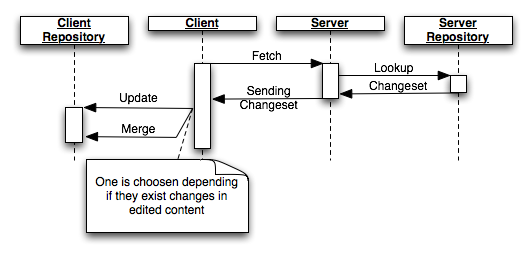
\includegraphics[scale=0.6]{charts/seq_update.png}
\caption{The pull operation sequence diagram.}
\label{fig:seq_update}
\end{center}
\end{figure}
The operation is started by the client by requesting changesets from the server and finishes after update or merge operation is performed on the client repository. As noted on figure~\ref{fig:seq_update} the condition deciding which of them should be chosen depends on existence of changes in the edited content. If merging is not needed then the update operation is done. When no chengsets are found then none of this is needed. That is a general rule when choosing between merge and update and for this reason that note wont be repeated on the following figures. It is also in common that on the sequence diagrams the client and server repository were separated from their version control repositories. By this concept front-end and back-end functions could be presented simultaneously. 

Figures~\ref{fig:seq_commit} and~\ref{fig:seq_commit2} are the product of  dissertation on what sequence of operations should be called to get a updated version after applying changes. The first one illustrates an idea of performing a \texttt{pull} first after the changes are saved in the clients repository and the \texttt{push} a the end of sequence. The opposite order is presented on figure~\ref{fig:seq_commit2} where \texttt{pull} is followed by \texttt{push}. 
\begin{figure}[ht]
\begin{center}
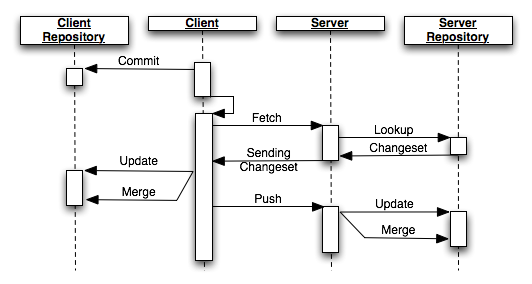
\includegraphics[scale=0.6]{charts/seq_commit.png}
\caption{The commit operation together with pull preceding the push operation.}
\label{fig:seq_commit}
\end{center}
\end{figure}
\begin{figure}[ht]
\begin{center}
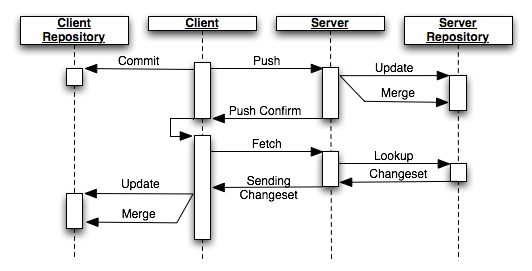
\includegraphics[scale=0.6]{charts/seq_commit2.png}
\caption{The commit operation that makes push follow the pull operation.}
\label{fig:seq_commit2}
\end{center}
\end{figure}
\newline Both of those attempts have its advantages and disadvantages. On balance the first concept appears to outperform the second one by characteristics:
\begin{itemize}
\item{The basic client action gets faster finished as it only saves the changes in the client repository.}
\item{Lower probability that the server will need to perform the merge operation. That allows to save the CPU resources and makes the application more scalable as the merges are done on the client application side. That also to solve eventual conflicts before the changesets will reach the server.}
\item{Better user experience as an effect that the changes are available in the interface offered by the client application sooner.}
\end{itemize}
From the other side the second concept ay seem more reliable as it gives grater priority to saving changesets both in the client and server repositories and preforms commit and \texttt{push} as the fist ones. That makes not that a big difference in practice and gets outweigh by the arguments mentioned above.




\subsection{iSmartNotes activation process}\label{subsec:ismartnotes_activation}
 
\chapter{System Evaluation}\label{chap:eval}
\section{Final result presentation}\label{sec:result} 
\section{Performance tests}\label{sec:performance}  

%\include{Conclusion}     %% Honors theses are required to 
                          %% have an unnumbered chapter
                          %% for conclusions.  The file
                          %% Conclusion.tex should begin
                          %%   
                          %% \chapter*{Conclusion}
                          %% followed by the appropriate
                          %% text.

%-->\include{biblio}            %% Calls biblio.tex.  See below.
%-->\Appendix                 %% Use this command if you have one 
                          %% appendix. Use \Appendices if you 
                          %% have more than one.
	
%-->\include{toolong}         %% Calls toolong.tex which contains
                          %% an appendix.


\end{document}
